\section{Auswertung}
\label{sec:Auswertung}

\subsection{Auf- und Entladevorgang des Kondensators}
\begin{table}[H]
  \centering
  \caption{Messwerte zur Auf- und Entladung des Kondensators}
  \label{tab:data1}
  \sisetup{table-format=2.1}
  \begin{tabular}{S S S}
    \toprule
    {$t$}&{$U_\text{Aufladung}$}&{$U_\text{Entladung}$} \\
    {$/[s]$}&{$/[V]$}&{$/[V]$} \\
    \midrule
    0   &  0.5 & 19   \\
    0.4 &  5   & 15   \\
    0.8 &  8   & 11.5 \\
    1.2 & 11.5 &  8   \\
    1.6 & 13   &  6.2 \\
    2   & 14.5 &  4.5 \\
    2.4 & 16   &  3.2 \\
    2.8 & 17   &  2.1 \\
    3.2 & 17.7 &  1.5 \\
    3.6 & 18   &  1.2 \\
    4   & 18.6 &  1   \\
    4.4 & 18.8 &  0.8 \\
    4.8 & 18.9 &  0.5 \\
    5.2 & 19   &  0.4 \\
    5.6 & 19   &  0.3 \\
    6   & 19   &  0.3 \\
    6.4 & 19   &  0.3 \\
    6.8 & 19   &  0.3 \\
    7.2 & 19   &  0.3 \\
    \bottomrule
  \end{tabular}
\end{table}

\begin{figure}[H]
  \centering
  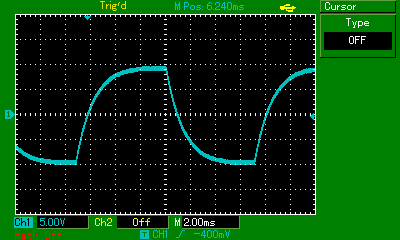
\includegraphics{content/images/a/ladekurve.png}
  \caption{Thermodruck auf und Entladung für eingehende Rechteckspannung.}
  \label{fig:lade}
\end{figure}
mit der Amplitude $U_0=$ \SI{20}{\volt}
\begin{figure}[H]
  \centering
  \includegraphics{build/zeitconst.pdf}
  \caption{Regressionsplot für den Auf- beziehungsweise Entladevorgang.}
  \label{fig:lade_plot}
\end{figure}
Regressionsgleichung für den Aufladevorgang nach \eqref{eqn:aufladen}
mit den Werten aus Tabelle \ref{tab:data1}:
\begin{equation}
  U(t)=b\left(1-e^{-t/a}\right)
\end{equation}
Aufladung:\\
$RC=a=$ \SI{1.388(30)e-3}{\second}\\
$b=$ \SI{19.378(108)}{\volt}\\\\
Regressionsgleichung für den Entladevorgang nach \eqref{eqn:entladen}
mit den Werten aus Tabelle \ref{tab:data1}:
\begin{equation}
  U(t)=b\left(e^{-t/a}\right)
\end{equation}
Entladung: \\
$RC=a=$ \SI{1.369(27)e-3}{\second}\\
$b=$ \SI{19.514(236)}{\volt}

\subsection{Amplituden in Abhängigkeit der Frequenz}
\begin{table}[H]
  \centering
  \caption{Messwerte zur relativen Amplitude und zur Phase}
  \label{tab:data2}
  \sisetup{table-format=1.3}
  \begin{tabular}{S[table-format=6.0] S[table-format=2.4] S S[table-format=1.5] S}
    \toprule
    {$\omega$}&{$A$}&{$A/U_0$}&{$\increment t$}&{$\phi$} \\
    {$/\pi [Hz]$}&{$/[V]$}&{}&{$/[s]$}&{$/rad$} \\
    \midrule
    200    & 13.8   & 0.742 & 1.32    & 0.829 \\
    300    & 11.1   & 0.597 & 1.12    & 1.056 \\
    600    & 6.44   & 0.346 & 0.68    & 1.282 \\
    800    & 5      & 0.269 & 0.528   & 1.327 \\
    1000   & 4.16   & 0.224 & 0.44    & 1.382 \\
    1500   & 2.7    & 0.145 & 0.32    & 1.508 \\
    2000   & 2.06   & 0.111 & 0.24    & 1.508 \\
    2400   & 1.74   & 0.094 & 0.184   & 1.387 \\
    3000   & 1.38   & 0.074 & 0.156   & 1.470 \\
    4000   & 1.02   & 0.055 & 0.116   & 1.458 \\
    10000  & 0.42   & 0.023 & 0.048   & 1.508 \\
    20000  & 0.21   & 0.011 & 0.0232  & 1.458 \\
    50000  & 0.084  & 0.005 & 0.0098  & 1.539 \\
    100000 & 0.042  & 0.002 & 0.00512 & 1.608 \\
    200000 & 0.0216 & 0.001 & 0.0028  & 1.759 \\
    \bottomrule
  \end{tabular}
\end{table}

\begin{figure}[H]
  \centering
  \includegraphics{build/amplituden.pdf}
  \caption{Regressionsplot für die Frequenzabhängigkeit der Amplitude.}
  \label{fig:amp_plot}
\end{figure}
unter beachtung von:
\begin{equation}
  \omega = 2\pi f
\end{equation}
Regressionsgleichung nach \eqref{eqn:amplitude}
mit den Werten aus Tabelle \ref{tab:data2}:
\begin{equation}
  \frac{A(\omega)}{U_0}=\frac{1}{\sqrt{1+a^2\omega^2}}
\end{equation}
$a=$ \pm\SI{1.422(5)e-3}{\second}\\
$RC=a_+=$ \SI{1.422(5)e-3}{\second}

\subsection{Phasen in Abhängigkeit der Frequenz}

\begin{figure}[H]
  \centering
  \includegraphics{build/phasen.pdf}
  \caption{Regressionsplot für die Frequenzabhängigkeit der Phase.}
  \label{fig:ph_plot}
\end{figure}

Regressionsgleichung nach \eqref{eqn:phase}
mit den Werten aus Tabelle \ref{tab:data2}:
\begin{equation}
  \text{sin}(\phi)=\frac{a\omega}{\sqrt{1+a^2\omega^2}}
\end{equation}
$RC=a=$ \SI{1.776(34)e-3}{\second}\\

\subsection{Amplituden-Phasen-relation}
Für die theoretische Kurve wird $RC=$ \SI{1.422(5)e-3}{\second} aus der Bestimmung durch die relativen
Amplituden $A/U_0$ gewählt:
\begin{figure}[H]
  \centering
  \includegraphics{build/polar.pdf}
  \caption{Regressionsplot für die Frequenzabhängigkeit der Phase.}
  \label{fig:pol_plot}
\end{figure}


\subsection{Integrabilität}
Nach \eqref{eqn:integral} muss die Kondensatorspannung proportional zum
Integral der Erregerspannung sein. In Abbildung \ref{fig:int_recht}
ist die Rechteckspannung als Erreger in blau sowie die
Kondensatorspannung in gelb aufgezeichnet. Bei der Rechteckspannung ist dieser
Zusammenhang einfach zu erkennen, da die Kondensatorspannung für eine
positive konstante Erregerspannung linear ansteigt und für eine
negative konstante Erregerspannung linear abfällt und es gilt:
\begin{align}
  x &\propto \int 1 d\, x &\text{beziehungsweise}&& -x &\propto \int -1 d\, x
\end{align}
\begin{figure}[H]
  \centering
  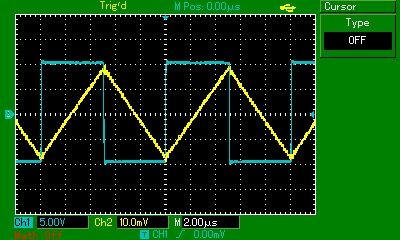
\includegraphics{content/images/d/rechteck.png}
  \caption{$U(t)$ in blau und $U_{\symup{c}}(t)$ in gelb für Rechteckspannung.}
  \label{fig:int_recht}
\end{figure}
In Abbildung \ref{fig:int_sin}
ist die Sinusspannung als Erreger in blau sowie die
Kondensatorspannung in gelb aufgezeichnet. Auch hier ist der Zusammenhang
gut zu sehen, da die Integration des Sinus den negativen Cosinus ergibt
welcher um \SI{90}{\degree} Phasenverschoben ist:
\begin{equation}
  \text{sin}(x-\SI{90}{\degree})=-\text{cos}(x) \propto \int \text{sin}(x)d\, x
\end{equation}
\begin{figure}[H]
  \centering
  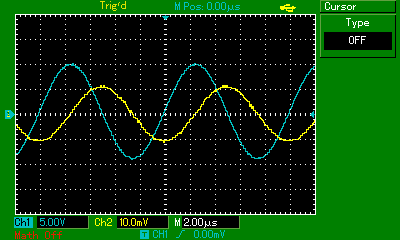
\includegraphics{content/images/d/sinus.png}
  \caption{$U(t)$ in blau und $U_{\symup{c}}(t)$ in gelb für Sinusspannung.}
  \label{fig:int_sin}
\end{figure}
In Abbildung \ref{fig:int_drei} ist die Dreiecksspannung
als Erreger in blau sowie die Kondensatorspannung in gelb aufgezeichnet.
Hier mag der Graph der Kondensatorspannung irreführender Weise zunächst
nach einem negativen Cosinus aussehen, bei näherer Betrachtung ist jedoch zu
erkennen, dass sich der Graph aus den Minima beziehungsweise Maxima
alternierend negativer und positiver Parabeln zusammensetzt.
Für die linear steigende Erregerspannung ergibt sich also das Minimum einer
nach oben geöffneten Parabel, für die linear fallende Erregerspannung
das Maximum einer nach unten geöffneten Parabel, wodurch die Integrabilität
auch für diese Erregerspannung gegeben ist:
\begin{align}
  x^2 &\propto \int x d\, x &\text{beziehungsweise}&& -x^2 &\propto \int -x d\, x
\end{align}
\begin{figure}[H]
  \centering
  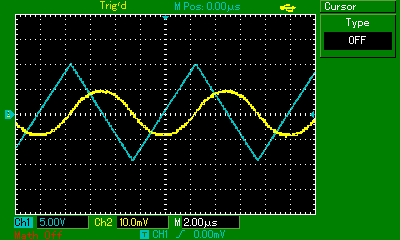
\includegraphics{content/images/d/dreieck.png}
  \caption{$U(t)$ in blau und $U_{\symup{c}}(t)$ in gelb für Dreiecksspannung.}
  \label{fig:int_drei}
\end{figure}
